\documentclass[../tp2_grupo404.tex]{subfiles}

\graphicspath{{\subfix{../out/}}}

\begin{document}

\subsubsection{Criterio de selección}

En el enunciado nos pide que el programa sirva para, con respecto a una nueva fábrica,
\textquote{determinar dónde la ubicarán para minimizar los gastos de logística y distribución}.
Pero también se indica que: \textquote{Cada ruta une dos depósitos en un
sentido. No todos los depósitos tienen rutas que los conecten}.

Así mismo se indica que se debe emplear el algoritmo de Johnson; éste
pruduce una tabla de distancias. Sin embargo, para emplearlo a tal fin es
necesario tomar una serie de decisiones relevantes para el criterio de selección,
a saber:
\begin{enumerate}
    \item Si todos los depósitos cuentan con la misma improtancia o si existe
    alguna ponderación.
    \item Con las condiciones dadas es posible encontrarse con la disyuntiva de
    acceder a pocos depósitos pero con mejor costo (incluso negativo) o elegir
    una opción con un costo más alto pero con acceso a más depósitos (aunque aun
    así no a todas).
\end{enumerate}

Para el primer punto, hemos asumido que todos cuentan con la misma importancia;
de lo contrario suponemos que se nos hubiera indicado que también se provee
una tabla de ponderaciones.

En cambio para el segundo entendemos que siendo una decisión con un posible
impacto considerable y que dependa de circunstancias más allá del modelo actual
(o, incluso, muy difíciles de modelar), le brindamos la información al usuario
para que tome la decisión con el criterio que considere preferibel.

Mientras que si hay al menos un vértice que llegue al máximo de nodos con el
mínimo costo, se tomará como la mejor recomendación (a pesar de que puedan
existir otros nodos con el mismo costo pero menos alcance o el mismo alcance
con mayor costo).

\begin{figure}[H]
    \centering
    \subcaptionbox
        {\label{grafoDisyuntiva}\textbf{Grafo de ejemplo que nos llevaría a la disyuntiva}}
        {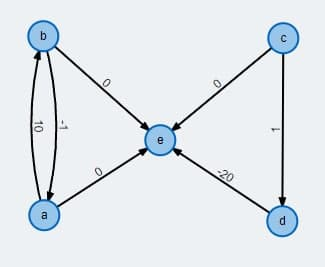
\includegraphics[width=0.4\linewidth,angle=0,origin=c]{img/disyuntiva.jpg}}
    \subcaptionbox
        {\label{outDisyuntiva}\textbf{Salida del programa, con y sin disyuntiva.}}
        {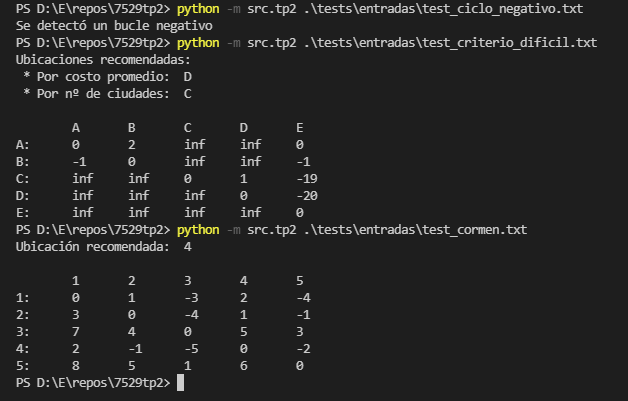
\includegraphics[width=0.4\linewidth,angle=0,origin=c]{img/salida.png}}
\end{figure}

Por ejemplo, para el caso del \cref{grafoDisyuntiva} si la fábrica se ubicara en
D tendría un costo promedio de -20 (es decir, genera ganancia), pero acceso a un sólo
depósito adicional; y si se ubica en C tiene un costo de -18, pero no puede alcanzar
a C ni D.

Entonces, será un usuario más conocdedor del problema quien podrá decidir si alguna de
las dos es una situación aceptable y cuál es preferible (¿cuál es el costo de no acceder
a ciertos depósitos?), o si sería preferible posponer la construcción de la fábrica y,
en ese caso, qué acciones se deben tomar; tales como crear una ruta, etc.

\subsubsection{Uso}
Para ejecutar el programa es necesario
\href{https://www.python.org/downloads/}{descargar e instalar Python 3.10}
y, desde la línea de comandos ubicado en la carpeta donde se descomprimió,
\footnote{}
ejecutar:
\begin{verbatim}
    python -m src.tp2 NOMBRE_DE_ARCHIVO
\end{verbatim}
Siendo \texttt{NOMBRE\_DE\_ARCHIVO} la ruta (relativa a la carpeta de trabajo)
al archivo con las rutas, según el formato indicado en
\hyperref[enuncFormatoArchivos]{Formato de archivos}.
Por ejemplo, para usarse el ejemplo dado en Cormen:
\begin{verbatim}
    python -m src.tp2 tests/entradas/test_cormen.txt
\end{verbatim}

\subsubsection{Explicación general de la implementación}

\newcommand{\ChangeLine}[1]{%
\ifodd\value{FancyVerbLine}%
\textcolor{gray}{#1}\else\textcolor{black}{#1}\fi}

\DefineVerbatimEnvironment{alternate}{Verbatim}{formatcom=\renewcommand{\FancyVerbFormatLine}{\ChangeLine}}{}

\begin{figure}[H]
    \centering
    \includestandalone[mode=tex,width=0.9\textwidth]{out/uml/dc/DCgeneral}
    \caption{\label{dcGeneral}Diagrama de clases general.}
    \end{figure}

Nos enfocaremos en los fragmentos del código más relevantes algorítmicamente.

\paragraph{src.Dijkstra}

\begin{alternate}[breaklines=true,numbers=left,xleftmargin=5mm]
    class Dijkstra:
    def __init__(self,grafo,desde):
        cantNodos = grafo.cantidadNodos()
        if (desde < 0) or (desde >= cantNodos):
            raise Exception("El nodo no existe")
        
        self._estadoVisitado = [False    for i in range(cantNodos)]
        self._visitables     = [i        for i in range(cantNodos)]
        self.distancias      = [math.inf for i in range(cantNodos)]
        self.distancias[desde] = 0
        
        while(len(self._visitables)):
            visitando = self._visitar()
            arcos = grafo.arcoDesdeNodoId(visitando)
            for(destino, peso) in arcos:
                if not self._fueVisitado(destino):
                    distanciaAlternativa = self.distancias[visitando] + peso
                    if distanciaAlternativa < self.distancias[destino]:
                        self.distancias[destino] = distanciaAlternativa

    def _visitar(self):
        # Ordenar visitables de menor a mayor distancia
        self._visitables = sorted(self._visitables, key=lambda nodo:self.distancias[nodo])

        aVisitar = self._visitables.pop(0)
        self._estadoVisitado[aVisitar] = True
        return aVisitar

    def _fueVisitado(self, nodo):
        return self._estadoVisitado[nodo]
\end{alternate}

\paragraph{src.BellmanFordConCeroAgregado}

Para el caso de Bellman-Ford, nos decidimos por una implementación sutilmente modificada, considerando que:
\begin{enumerate}
    \item Sólo se emplea dentro de Johnson.
    \item Se agrega un vértice de grado de entrada cero y con aristas de peso 0; pero se descarta al finalizar.
    \item Dentro del algoritmo no se modifica el grafo más allá del punto anterior.
\end{enumerate}

En particular, se optó por evitar crear una copia del grafo o tener que modificarlo. Algunas observaciones al respecto:
\begin{enumerate}
    \item[13] Se agregaría una arista por nodo preexistente. En vez de eso, simplemente se calcula la cantidad.
    \item[20] Se inicializa en 0 porque siempre será el resultado al iterar por primera vez por las aristas agregadas.
    \item[22] Tal como se establece en el algoritmo se itera externamente una vez por cada vértice del grafo modificado.
    \item[25] Se implementa una parada temprana: en caso de que no haya modificaciones, cada iteración terminará con el mismo resultado.
    \item[28] Por claridad la detección de bucles negativos se especificó externamente.
    Si bien, como hay detección de cambios en la iteración interna podría hacerse una iteración más y si sale del bucle
    con cambios, encontró un bucle negativo.
    \item[33] Aquí está la parte de la iteración interna por cada arista.
\end{enumerate}

\begin{alternate}[breaklines=true,numbers=left,xleftmargin=5mm]
    class BellmanFordConCeroAgregado:
    def __init__(self,grafo):
        """Crea una instancia con las distancias para un grafo copia del
        dado, al que se añade un nodo con arcos de peso 0 hacia el resto
        de los nodos (pero sin nodo que llegue al mismo). Las distancias
        serán calculandas con Bellman-Ford¹ para el nodo agregado, pero
        sólo se devolverá las de los demás nodos.
        ¹ Sabiendo que el nodo agregado no tiene nodos de entrada por lo
        que no puede cambiar su distancia, y entonces desde ella hasta
        otros siempre será 0, en esta implementación no se almacena."""
        cantNodos = grafo.cantidadNodos()
        cantArcosCon0 = grafo.cantidadArcos() + grafo.cantidadNodos()
        self._arcos = list(grafo.arcos())

        if cantNodos<1:
            raise Exception("")
        # En la primera iteración real de Beellman-Ford, como el nodo
        # agregado tiene arcos de peso 0, todos pasan a tener esa distancia.
        self.distancias = [0 for i in range(cantNodos)]

        for k in range(cantArcosCon0 - 1):
            self._iterar()
            # Finalización temprana:
            if(not self._huboCambio):
                break

        # Comprobar bucle
        self._iterar()
        if(self._huboCambio):
            self.distancias = False

    def _iterar(self):
        self._huboCambio = False
        for (origen,destino,peso) in self._arcos:
            distanciaAlternativa = self.distancias[origen] + peso
            if distanciaAlternativa < self.distancias[destino]:
                self.distancias[destino] = distanciaAlternativa
                self._huboCambio = True
\end{alternate}

\paragraph{src.Johnson}

\begin{enumerate}
    \item[9] Aquí verificamos que haya algún peso negativo, para aplicar la transformación si es necesaria:
    \item[10] Se obtienen las distancias al nodo temporal con Bellman-Ford.
    \item[11] Se modifica el grafo con la fórmula $\hat{w} = w + h(u) - h(v)$.
    \item[13] En caso de que no se haya aplicado ninguna modificación, se deja $h$ en cero.
    \item[19] Aquí se aplica la corrección si se modificó (en caso contrario, es 0).
\end{enumerate}

\begin{alternate}[breaklines=true,numbers=left,xleftmargin=5mm]
    from src.bellmanford import BellmanFordConCeroAgregado
    from src.dijkstra import Dijkstra
    
    class Johnson:
        def __init__(self, grafo):
            if grafo.cantidadNodos()<1:
                raise Exception("No hay suficientes nodos")
    
            if any(peso<0 for (u,v,peso) in grafo.arcos()):
                h = BellmanFordConCeroAgregado(grafo).distancias
                grafo.modificarPesos( lambda w,u,v: w +h[u] -h[v] )
            else:
                h = [0 for i in range(grafo.cantidadNodos())]
            self.h = h
            
            self.matriz = []
            for u in range(grafo.cantidadNodos()):
                d = Dijkstra(grafo, u).distancias
                self.matriz.append([ d[v] + h[v] -h[u] for v in range(grafo.cantidadNodos()) ])
\end{alternate}

% FIN DEL DOCUMENTO (SECCIÓN P1.7)
% NO BORRAR POR ACCIDENTE NI ESCRIBIR COSSA ABAJO
\end{document}
